%!TEX root = ../dokumentation.tex

\chapter{Umsetzung}

Nachdem der Schritt der Planung und der Analyse abgeschlossen ist, kann nun mit
der tatsächlichen Entwicklung fortgefahren werden. Dazu müssen zunächst die einzelnen
Entwicklungsumgebungen vorbereitet werden und die ersten Konzepte für
die Umsetzung aufgestellt und abschließend realisiert werden.

\section{Voraussetzungen}
Um mit der Entwicklung des Audioplayers beginnen zu können, müssen zunächst
einige Anpassungen und Installationen getätigt werden. Diese Schritte sind
notwendig, damit die zu verwenden Bibliotheken wie vorgesehen funktioniert und
keine ungewollten Zustände entstehen.

\subsection{Pakete installieren und Raspberry Pi updaten}
Standardmäßig besitzt der Raspberry Pi das Betriebssystem \textit{Raspbian}.
Dieses gilt es zuerst auf die neuste Version zu aktualisieren. Zusätzlich
sollten alle installierten Pakete des System auf die neuste Version aktualisiert
werden. Dies kann durch die folgenden Befehle durchgeführt werden:
\begin{lstlisting}[caption={Aktualisieren des Raspberry Pi}]
sudo apt-get update 
sudo apt-get upgrade 
sudo apt-get install rpi-update 
sudo rpi-update
\end{lstlisting}
Die ersten drei Befehle werden mit \ac{APT} ausgeführt. \ac{APT} ist ein
Paketverwaltungssystem, welches für den Bereich der Debian Betriebssysteme
entwickelt wurde. Da Raspbian ein debian-basiertes Betriebssystem ist, können
die installierten Pakete des Raspberry Pis durch \ac{APT} verwalten werden
\autocite{apt-debian-wiki_2019}. Zusätzlich wird für alle durchzuführende
Befehle der \verb|sudo| Befehl benutzt. \ac{Sudo} wird benutzt, um
bestimmte Befehle mit Root-Rechten (Administratorrechten) auszuführen.
\ac{Sudo} bietet den Vorteil, dass man nicht zum Administrator-Account wechseln
muss, um kurz einen Befehl mit dessen Privilegien auszuführen
\autocite{moeller_2013}. Mit dem Befehl \verb|sudo apt-get update| werden alle
Paketquellen neu eingelesen. Dafür wird ein Abgleich zu einem externen Lexikon
gemacht, in welchem zu jedem Paket die aktuellste Versionsnummer steht. Wenn
sich die lokal installierte Versionsnummer von der externen Liste
unterscheidet, lädt der Befehl den Link zur neuesten Version runter.
Mit dem Befehl \verb|sudo apt-get upgrade| wird mit den durch den vorherigen
Befehl erhaltenen Links zu den neuen Paketversionen die aktualisierten
Versionen dieser Pakete heruntergeladen und installiert. Die Installation von
neuen Abhängigkeit oder die Löschung nicht mehr benötigter Abhängigkeiten wird
durch diesen Befehl nicht vollzogen \autocite{apt-get-wiki_2019}. Mit dem Befehl
\verb|apt-get install rpi-update| wird das Paket \verb|rpi-update| mit all
seinen Abhängigkeiten heruntergeladen und installiert. Das Paket ist ein
automatisiertes Skript, welches das Betriebssystem des des Raspberry Pi's auf die
neuste Version aktualisiert. Als letzten Schritt wird das Paket \verb|rpi-update|
ausgeführt, wodurch die tatsächliche Aktualisierung des Betriebssystems gestartet wird.
\newline 
Im nächsten Schritt müssen folgende Pakete installiert werden, um später die
Audiowiedergabe zu ermöglichen. 
\begin{lstlisting}[caption={Installation benötigter Pakete}]
sudo apt-get install portaudio19-dev
sudo apt-get install libmpg123-dev
sudo apt-get install mp3info 
\end{lstlisting}

\subsection{Schritte zur Einrichtung der Entwicklungsumgebung}
Im Folgenden werden alle erforderlichen Schritte erläutert, welche zur
Entwicklung des Audioplayers vonnöten sind.

\subsubsection{Installieren von Go}
Nun wird auf die Installation von Go eingegangen.

\begin{enumerate}
\item \textbf{Herunterladen von Go} \\
Im ersten Schritt gilt es die Programmiersprache Go auf den Raspberry Pi
herunterzuladen. Dazu stellt der Hersteller offizielle Pakete für die
unterschiedlichen Betriebssysteme und Architekturen zum Download bereit. Diese
können über die \href{https://golang.org/dl/}{Download-Webseite}
heruntergeladen werden. In diesem Fall wird für den Raspberry Pi das Paket für
das Betriebssystem \textit{Linux} mit der Architektur \textit{ARMv6} benötigt.
Nachdem das passende Paket auf der Webseite gefunden wurde, muss der
Direkt-Link zu dem Download in den Zwischenspeicher kopiert werden und
anschließend der folgende Befehl auf dem Raspberry Pi ausgeführt werden.
\begin{lstlisting}[caption={Herunterladen einer Datei}]
Befehl: wget [LINK]
\end{lstlisting}

\item \textbf{Entpacken des Archivs} \\
Nachdem das offizielle Archiv für die Programmiersprache Go heruntergeladen
wurde, muss dieses in den Pfad \verb|/user/local| extrahiert werden. Für
das Entpacken des Archivs wird das standardmäßige Archivierungsprogramm für
Linux \textit{\ac{Tar}} verwendet. Der große Vorteil eines \ac{tar}-Archivs ist,
dass die Benutzerrechte einer Datei mitgesichert werden und diese beim
Entpacken auch wiederhergestellt werden \autocite{tar-wiki_2019}. Das Entpacken
des Archivs wird durch den Befehl im Listing \ref{lst:extract_with_tar}
realisiert. Der Dateiname entspricht hier der zuvor heruntergeladenen Datei.
\begin{lstlisting}[caption={Entpacken eines Archivs},label={lst:extract_with_tar}]
tar -C /usr/local -xzf [Filename]
\end{lstlisting}

\item \textbf{Setzen des Export-Pfad} \\
Damit das Betriebssystem den Befehl \verb|go| systemweit kennt, muss der Pfad zu der
ausführbaren Datei von Go zu der PATH-Variable hinzugefügt werden. Die
\textit{PATH-Variable} ist eine Umgebungsvariable, die aus einer
Komma-separierten Liste von Ordnern besteht, welche die Shell bei der Eingabe
eines Kommandos durchsucht \autocite{quigley_2000}. Dies bewirkt, dass von
jedem Standort im System auf Go bzw. den Go Compiler zugegriffen werden kann.
\begin{lstlisting}[caption={Setzen der Go-Path Variable}]
export PATH=\$PATH:/usr/local/go/bin
\end{lstlisting}

\item \textbf{Überprüfen der Go Installation auf Korrektheit} \\
Um zu überprüfen, ob Go richtig installiert und die Path-Variable
korrekt gesetzt wurde, wird nun durch den Befehl \verb|go version|
eine Abfrage an den Go Compiler zu seiner aktuellen Version erstellt. Falls der
Befehl keinen Fehler wirft und die Ausgabe die Versionsnummer der
Go-Installation anzeigt, wurde Go korrekt installiert und im System
integriert.
\begin{lstlisting}[caption={Go Version anzeigen}]
go version -> "go version go x.x.x"
\end{lstlisting}

\item \textbf{Go-Ordnerstruktur anlegen} \\
Go empfiehlt eine bestimmte Ordnerstruktur für die Go Projekte anzulegen.
Die empfohlene Ordnerstruktur sieht wie folgt aus:
\begin{itemize}
\item \textbf{bin} - enthält alle Go-Executable's, die mit dem Befehl \verb|go install| installiert wurden.
\item \textbf{pkg} - enthält alle kompilierten Pakete, die in Projekte importiert werden können. 
\item \textbf{src} - enthält alle Quelldateien, entweder die eigenen oder aus externen Repositories heruntergeladene Quellen.
\end{itemize}
In der folgenden Übersicht wird die Ordnerstruktur nochmals visuell
dargestellt. Der Ordner \textit{pi} stellt hier den Nutzernamen da, welcher im
Betriebssystem hinterlegt ist. \newline
\begin{minipage}[t]{\textwidth}
\begin{figure}[H]
\dirtree{%
.1 /. 
.2 home. 
.3 pi. 
.4 go. 
.5 src. 
.5 pkg. 
.5 bin. 
}
\caption{Ordnerstruktur von Go} 
\end{figure}
Die Befehle zur Erstellung der Ordnerstruktur sehen wie folgt aus. \\
Ausgehend von \verb|$Home|:
\begin{lstlisting}[caption={Erstellung der Go Ordnerstruktur},label={lst:go_folder_structure}]
mkdir go
cd go
mkdir src
mkdir pkg
mkdir bin
\end{lstlisting}
\end{minipage}


\end{enumerate}

\subsubsection{Klonen des Git Repository}
Der nächste Schritt ist das Git Repository auf den lokalen PC zu klonen. Go
schreibt dafür einen Standard vor, wie die Ordnerstruktur dazu bestenfalls
aufgebaut werden sollen. Im Folgenden werden nun die Befehle zur Erstellung der
Ordnerstruktur dargestellt. Diese Befehle Starten von \verb|/home/pi/go/src/|:
\newpage
\begin{lstlisting}[caption={Klonen des Git Repository}]
mkdir github.com 
cd github.com
mkdir alexanderklapdor
cd alexanderklapdor
git clone https://github.com/alexanderklapdor/RaspberryPi_Go_Audioplayer.git
\end{lstlisting}

\subsubsection{Installieren der Go Abhängigkeiten}
Bei der Entwicklung des Audioplayers wurden weitere Go-Projekte verwendet,
welche nun für die Entwicklung auf den lokalen Rechner heruntergeladen werden
müssen. Um nicht alle Abhängigkeiten einzeln zu installieren, kann Go sich alle
benötigten Projekte alleine herunterladen. Dies wird durch den folgenden Befehl
gemacht.
Ausgehend von \verb|../RaspberryPi_Go_Audioplayer/| :
\begin{lstlisting}[caption={Installieren von Go Abhängigkeiten}]
go get ./... 
\end{lstlisting}

\subsubsection{Modifizieren der \acs{ALSA} Bibliothek Dateien}
Die Konfigurationsdatei der \acf{ALSA} Bibliothek muss editiert werden, damit die
Fehlermeldungen, welche durch die nicht vorhandenen Anschlüsse am Raspberry Pi
hervorgerufen werden, nicht immer mit ausgegeben werden. \\
Die Datei kann durch den Befehl \verb|sudo nano /usr/share/alsa/alsa.conf| aufgerufen werden. \newline
Folgende Einträge müssen aus dieser Datei entfernt werden:
\begin{lstlisting}[caption={Liste der zu löschenden Einträge}]
pcm.rear cards.pcm.rear 
pcm.center_lfe cards.pcm.center_lfe 
pcm.side cards.pcm.side 
pcm.surround21 cards.pcm.surround21 
pcm.surround40 cards.pcm.surround40 
pcm.surround41 cards.pcm.surround41 
pcm.surround50 cards.pcm.surround50 
pcm.surround51 cards.pcm.surround51 
pcm.surround71 cards.pcm.surround71 
pcm.iec958 cards.pcm.iec958 
pcm.spdif iec958 
pcm.hdmi cards.pcm.hdmi 
pcm.dmix cards.pcm.dmix 
pcm.dsnoop cards.pcm.dsnoop 
pcm.modem cards.pcm.modem 
pcm.phoneline cards.pcm.phoneline
\end{lstlisting}

\subsection{Nötige Schritte für die Nutzung}
Für die reine Nutzung des Audioplayers sind nur weniger Schritte notwendig,
da eine bereits kompilierte Version heruntergeladen und genutzt werden kann.
Dazu sind folgende Schritte notwendig:
\begin{enumerate}
\item \textbf{Herunterladen der neusten \href{https://github.com/alexanderklapdor/RaspberryPi_Go_Audioplayer/releases}{Release} Datei}  \\
\begin{lstlisting}[caption={Herunterladen einer Datei}]
wget [LINK]
\end{lstlisting}

\item \textbf{Entpacken des Archiv} \\
\begin{lstlisting}[caption={Entpacken eines Archivs}]
tar -xvf RaspberryPi_Go_Audioplayer_v***.tar
\end{lstlisting}

\item \textbf{Starten des Audioplayers} \\
\begin{lstlisting}[caption={Starten des Audioplayers}]
./RaspberryPi_Go_Audioplayer_v***/MusicPlayerClient
\end{lstlisting}
\end{enumerate}

\section{Konzept}
Um eine übergreifende Sicht über den Audioplayer zu bieten, werden in den
folgenden Abschnitten die einzelnen Konzepte für die Umsetzung dargestellt.
Dazu wird als erstes ein übergeordnetes Konzept dargestellt und erläutert,
um einen Überblick über die einzelnen Komponenten des entwickelten Audioplayers
zu erhalten.

\begin{figure}[h]
	\centering
	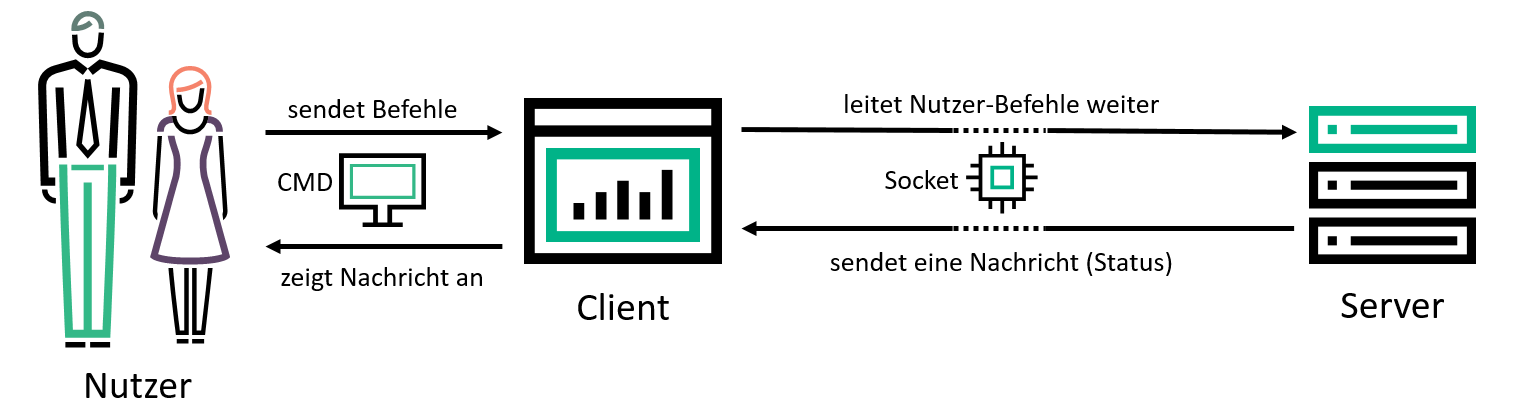
\includegraphics[scale=0.5]{Audioplayer_Konzept.png}
	\caption{Konzept des Audioplayer}
	\label{img:Konzept-Audioplayer}
\end{figure}

Das in Abbildung \ref{img:Konzept-Audioplayer} dargestellte Konzept spiegelt
eine übergreifende interaktive Sicht des Audioplayers wieder. Zudem sind in der
Abbildung alle für den Audioplayer benötigten Komponenten zu erkennen, wie:
\begin{itemize}
\item Nutzenden Personen
\item \ac{CMD}
\item Audioplayer-Client
\item Socket
\item Audioplayer-Server
\end{itemize}

Der Aufbau dieses Konzeptes wurde bewusst so gewählt, dass keine
Abhängigkeiten zwischen der Eingabe von Befehlen durch den Nutzer
und den technischen Funktionen des Audioplayers zur Wiedergabe und Steuerung
der Audiodateien besteht. Daher sind der Client und der Server eigenständige
Programme, die über einen Socket kommunizieren. Ein weiterer Vorteil dieses
Aufbaus ist, dass theoretisch mehrere Nutzer den selben Audioplayer steuern
können. \newline 
Die nutzenden Personen stellen den späteren Bediener des Audioplayers dar,
welche über ein Kommandozeilen-Programm (\ac{CMD} bzw. Shell) Befehle an den
Audioplayer-Client senden können. Die Befehle werden durch den Aufruf des
Client mit den entsprechenden Parametern übergeben. Der Client empfängt die
Befehle des Nutzers und leitet diese als \ac{JSON} über einen vorher
erstellten Socket an den Server weiter. Der Server interpretiert den Befehl und
führt die gewünschte Aktion aus. Anschließend sendet der Server eine
Statusmeldung (Nachricht) an den Client zurück, welcher diese dem Nutzer über
das Kommandozeilen-Programm ausgibt. Danach beendet sich der Client
wieder, wohingegen der Server weiterläuft, bis dieser explizit durch einen
\enquote{Beenden} Befehl heruntergefahren wird. \\ 
Diese Beschreibung des Konzeptes stellt nur eine grobe Übersicht der
Funktionsweise dar, weshalb in den nächsten Kapiteln nochmals genauer auf
den Client sowie den Server und den Socket eingegangen wird. Zusätzlich wird
die Nutzung von Konfigurationsdateien, sowie der Aufbau des Audioplayers
erläutert.

\subsection{Nutzung einer Konfigurationsdatei}
Unter einer Konfigurationsdatei versteht man eine
Klartext-Datei, in welcher Einstellungen für Computerprogramme gespeichert
werden. Für die Speicherung einer Konfigurationsdatei werden viele
unterschiedliche Formate wie z.B.  \ac{INI}, \ac{YAML}, \ac{XML} oder \ac{JSON}
verwendet \autocite{hard_coding_and_soft_coding_2019} \autocite{lott_2019}. \\ 

Für den erstellten Audioplayer wurde eine Konfigurationsdatei in dem Format
\ac{JSON} verwendet, um wichtige Einstellungen verändern zu können, ohne 
den Programmcode verändern zu müssen. Aus diesem Grund wurden folgende
Einstellungsmöglichkeiten innerhalb der \ac{JSON}-Konfigurationsdatei festgesetzt.
\begin{lstlisting}[language=Json,caption={Konfigurationsdatei des Audioplayers},label={lst:kommfick}]
{
"Socket_Path" : "/tmp/mp.sock",
"Log_Dir": "logs/",
"Server_Log": "server.log",
"Server_Connection_Attempts": 10,
"Client_Log": "client.log",
"Default_Command": "default",
"Default_Depth": 2,
"Default_Input": "",
"Default_Loop": true,
"Default_Shuffle": false,
"Default_Volume": 50,
"Debug_Infos": true
}
\end{lstlisting}

Wie in dem Ausschnitt  der Konfigurationsdatei im Listing \ref{lst:kommfick}
klar zu erkennen ist, werden einige Standardwerte für den Audioplayer in der
Konfigurationsdatei gespeichert, wie unter anderem den \enquote{Loop} und
\enquote{Shuffle} Status, die Standardlautstärke oder auch die Tiefe für das
Durchsuchen von übergebenen Ordnern. Zusätzlich werden dort die
Dateien bzw. Ordner angegeben, in denen unter anderem der Socket erstellt
oder die Log Dateien gespeichert werden sollen. Besonders zu
erwähnen ist, dass man über das Feld \verb|Debug_Infos| steuern kann, ob bei
der Ausführung des Audioplayers Debug-Informationen mit ausgegeben werden
sollen oder nicht. Dies ist gerade bei der weiteren Entwicklung des
Audioplayers von hoher Relevanz.

\subsection{Aufbau des Audioplayers}
Go besitzt einige Kodierrichtlinien, die dazu führen, dass der geschriebene
Programmcode möglichst kurz, einfach und strukturiert ist. Um genau das zu
erreichen, besitzt Go die Kodierrichtlinie zur Verwendung von sogenannten
\textit{Packages}, welche zusammengehörigen Programmcode in eine extra Datei
bzw. einem Package auslagert. In Go ist jeder Programmcode einem Package
zugeordnet. So ist z.B. das Hauptprogramm, also das Programm welches beim
starten eines Go-Programmes aufgerufen wird, immer im \enquote{main}-Package.
Sobald es einige zusammengehörige Funktionen, sei es sinngemäß oder für
einen gewissen Zweck, in ein Package ausgelagert werden können, soll dies gemacht werden.
Für jedes erstellte Package wird ein eigener Ordner in dem Verzeichnis
angelegt, indem alle zu dem Package zugehörige Dateien gespeichert werden.
Dabei kann ein Package aus mehreren Dateien bestehen, die mehrere Funktionen
exportieren oder aus nur einer Datei, die nur eine Funktion exportiert.
Zusätzlich sollte die Namenskonvention für Packages möglichst kurz, aber
dennoch verständlich sein \autocite{crawshaw_2019}. \\
Der Aufbau des Audioplayers wurde auf Basis dieser Kodierrichtlinie erstellt,
sodass sich die folgende Ordnerstruktur ergibt:
\begin{figure}[H]
\dirtree{%
.1 /. 
.2 logger. 
.3 logger.go. 
.2 portaudiofunctions. 
.3 portaudiofunctions.go.
.2 screener. 
.3 screener.go. 
.2 sender. 
.3 sender.go.
.2 serverfunctions. 
.3 audiofunctions.
.4 audiofunctions.go.
.3 connectionfunctions.
.4 connectionfunctions.go.
.3 volumefunctions.
.4 volumefunctions.go.
.2 structs.
.3 structs.go.
.2 util.
.3 util.go.
.2 config.json.
.2 MusicPlayerClient.go.
.2 MusicPlayerServer.go.
}
\caption{Ordnerstruktur des Audioplayers} 
\end{figure}

Die Hauptprogramme, also der Server und der Client, sowie die erstellte
Konfigurationsdatei liegen im \textit{Root-Verzeichnis} des Audioplayers. Wie
zu erkennen, stellen die restlichen Ordner mit den beinhaltenden Dateien
jeweils einzelne Packages dar, die von Go-Programmen aufgerufen werden können. \\
Folgend wird jedes Package kurz beschrieben:  
\begin{enumerate}
\item \textbf{logger-Package} \\
Dieses Package wird von fast allen Funkionen des Audioplayers zur Erstellung
von Log-Dateien genutzt. Zudem bietet es auch Funktionen zur Initialisierung des
Loggers.

\item \textbf{portaudiofunctions-Package} \\
In diesem Package sind alle Funktionen, die für die Verwendung der
PortAudio-Bibliothek notwendig sind, vorhanden. 


\item \textbf{screener-Package} \\
Das screener-Package besitzt Funktionen, welche den Nutzer einen Start- und
Endbildschirm bei der Verwendung des Audioplayers anzeigt.


\item \textbf{sender-Package} \\
Das sender-Package beinhaltet die Funktionen zum Senden und Empfangen von
JSON-Nachrichten für den Client über den Socket.


\item \textbf{audiofunctions-Package} \\
Innerhalb des audiofunctions-Package befinden sich Funktionen, welche für das
Abspielen von Audiodateien vonnöten sind.

\item \textbf{connectionfunctions-Package} \\
Hier sind die Funktionen für das Erstellen sowie das Senden, Empfangen und
Schließen des Sockets hinterlegt. Dies wird für den Kommunikation zwischen
Client und Server benötigt.

\item \textbf{volumefunctions-Package} \\
Durch dieses Package kann die Lautstärke für die Wiedergabe von Audiodateien
verändert werden.

\item \textbf{structs-Package} \\
Um auf die gleichen Strukturen vom Client und Server zugreifen zu können,
wurden diese in dem Package Struct ausgelagert.

\item \textbf{util-Package} \\
In diesem Package befinden sich sämtliche Grundfunktionen, die meist von
mehreren Packages genutzt werden. Zum Beispiel enthält sie eine Funktion, die
Strings nach einer bestimmten Zeichenkette durchsucht.
\end{enumerate}



\subsection{Konzept des Clients}
Wie bereits zuvor erläutert, hat der Client die Aufgabe die Befehle für den
Audioplayer vom Nutzer entgegenzunehmen und diese an der Server über einen
Socket weiterzuleiten.

\begin{figure}[H]
    \begin{struktogramm}(160,75)[Main-Funktion] 
        \assign{\hfill Konfigurationsdatei auslesen\hfill} 
        \assign{\hfill Aufsetzen des Loggers\hfill}
        \ifthenelse[12]{2}{1} {Überprüfen ob Server bereits läuft}{Ja}{Nein} 
        	\change
            \assign[5]{\hfill Starten des Servers\hfill}
        \ifend
        \ifthenelse[15]{2}{1} {Überprüfen ob Übergabeparameter vorhanden sind}{Ja}{Nein} 
        	\assign{\hfill Parsen der Informationen in ein \ac{JSON}-Format\hfill}
            \assign{\hfill Senden des \acp{JSON} an den Server\hfill}
            \while[5]{Bis Nachricht vom Server kommt}
            	\assign{\hfill Warten...\hfill}
            \whileend
            \assign{\hfill Anzeigen der Nachricht vom Server\hfill}
            \change
        \ifend
        \assign[5]{\hfill Beenden des Clients\hfill}
    \end{struktogramm} 
\caption{Programmablauf des Clients} 
\label{lst:client_ablauf} 
\end{figure}

In der Abbildung \ref{lst:client_ablauf} wird der Programmablauf des Clients in
einem Struktogramm dargestellt und nachfolgend kurz erörtert. Als ersten Schritt ließt
der Client die zuvor erläuterte Konfigurationsdatei ein und initialisiert
anschließend den Logger, um alle folgenden ausgeführten Aktionen im Client in
einer Logdatei zu protokollieren. Anschließend wird überprüft ob ein Prozess
des Serverprogramms bereits existiert und läuft. Falls dies nicht der Fall ist,
startet der Client das Serverprogramm und wartet bis der Server hochgefahren
ist und eine Verbindung zum Server besteht. Sobald eine
Verbindung besteht, wird überprüft, ob Übergabeparameter bei dem Aufruf des
Clients übergeben wurden. Wurden keine Parameter übergeben, wird eine
Statusmeldung angezeigt und das Clientprogramm beendet sich. Falls jedoch
Parameter übergeben worden sind, werden diese Informationen (Befehle) in ein
\ac{JSON}-Format geparst und anschließend über den Socket an den Server
gesendet. Der Client wartet bis er eine Antwort vom Server bekommt, in welcher
der Server eine Statusmeldung zurückgibt.  Die Statusmeldung wird dem Nutzer
angezeigt und der Client beendet sich anschließend automatisch.

\subsection{Konzept des Servers}

Der Server stellt das \enquote{Herz} des Audioplayers dar. Nach einmaligem
starten des Servers läuft dieser permanent als Prozess im Hintergrund und
setzt die Funktionen des Audioplayers um.

\begin{figure}[H]
    \begin{struktogramm}(160,80)[Main-Funktion] 
        \assign{\hfill Konfigurationsdatei auslesen\hfill} 
        \assign{\hfill Aufsetzen des Loggers\hfill}
        \assign{\hfill Aufsetzen des Sockets\hfill}
        \while[5]{Endlosschleife}
        	\assign{\hfill Abhören des Sockets auf Nachrichten\hfill}
        	\ifthenelse[12]{5}{1} {Nachricht erhalten}{Ja}{Nein}
        	    \assign[5]{\hfill Entpacken der Nachricht\hfill}
        	    \ifthenelse[12]{6}{5} {Befehl == \enquote{Beenden}}{Ja}{Nein}
        	    	\assign[5]{\hfill Nachricht an Client senden\hfill}
        	    	\assign[5]{\hfill Beenden der Wiedergabe\hfill}
        	    	\assign[5]{\hfill Schließen des Sockets\hfill}
        	    	\assign[5]{\hfill Beenden des Servers\hfill}
        	    	\change
        	    	\assign[10]{\hfill Ausführen des Befehls\hfill}
        	    	\assign[10]{\hfill Nachricht an Client senden\hfill}
        	    \ifend
        		\change
        	\ifend
        \whileend
    \end{struktogramm} 
\caption{Programmablauf des Servers} 
\label{lst:server_ablauf} 
\end{figure}

In der Abbildung \ref{lst:server_ablauf} wird der grobe Programmablauf des
Server dargestellt. Nachfolgend wird das Konzept nochmal kurz erläutert.
\newline
Im ersten Schritt liest der Server, genau wie der Client, die
Einstellungen aus der Konfigurationsdatei aus und setzt anschließend den Logger
zum Protokollieren der entstehenden Ereignisse auf. Anschließend setzt der
Server den Socket für die Kommunikation mit dem Client auf, wozu er den in der
Konfigurationsdatei festgelegten Pfad zur Erstellung des
Kommunikationsendpunktes nutzt. Sobald der Socket aufgesetzt ist und läuft,
wartet der Server in einer Endlosschleife auf einen Befehl des Clients und
durchläuft dabei folgende Schritte: \newline
Falls eine Nachricht durch den Client eingetroffen ist, wird die
eingetroffene Nachricht, welche in einem \ac{JSON} Format vorliegt,
geparst, um die darin liegenden Informationen auslesen zu können. Im Falle
dessen, dass als Befehl das Beenden des Server ankommt, wird zuerst eine
Bestätigungsnachricht an den Client geschickt. Falls aktuell eine Wiedergabe
durchgeführt wird, wird diese beendet. Danach wird der Socket geschlossen und
das Serverprogramm beendet. Bei jedem anderen Befehl wird die gewünschte Aktion
durchgeführt und nach erfolgreicher Ausführung eine Statusmeldung an den Client
zurück gesendet.
	

\section{Kommunikation über Sockets}
Die größte Schwierigkeit bei dem Projekt ist es, ein Programm zu entwickeln,
welches die Steuerung von Audiodateien ermöglicht, aber gleichzeitig noch in
der Lage ist, Befehle durch den Nutzer entgegen zu nehmen. Im Zuge dessen
fiel die Entscheidung auf das zuvor benannte
Client-Server-Modell. Um die Kommunikation dieser beiden zu ermöglichen, wurde
sich für den Einsatz von einem Socket entschieden. \newline
Ein \textit{Socket} ist ein Kommunikationsendpunkt, der vom Betriebssystem als
Objekt bereitgestellt wird. Programme verwenden meistens Sockets, um mit anderen
Programmen Daten auszutauschen und miteinander zu kommunizieren. Dies ist
unabhängig davon, ob beide Programme sich auf dem selbem Computer oder einem
anderen, über das Netzwerk erreichbaren Computer, befinden. Sockets
kommunizieren in der Regel bidirektional, was bedeutet, dass über den Socket
sowohl Daten gesendet wie auch empfangen werden können. Technisch ist der
Socket ein Speicherbereich, indem Konfigurationsparameter einer Verbindung, wie
auch ankommende und abgehende Daten zwischengespeichert werden. Aufgrund
dessen, dass ein Socket vom Betriebssystem bereitgestellt wird, hat man keinen
direkt Zugriff auf den Socket, sondern kann nur über Funktionen der
Programmiersprache auf den Socket zugreifen \autocite{pollakowski_2012}. \\
Diese Kommunikation erlaubt es, dass der Server im Hintergrund Befehle entgegennehmen und
Audiodateien abspielen kann, ohne dass das System "blockiert". 

\section{Funktionen des Audioplayers}
Nach der Beschreibung der Konzepte zur Umsetzung des Audioplayers, 
wird nun auf die implementierten Funktionen des Audioplayers eingegangen. Dabei wird
zu jeder Funktion eine kurze Beschreibung sowie die Syntax für den Aufruf
erläutert.


\definecolor{Gray}{gray}{0.9}
\begin{longtable}{l|l} 
\rowcolor{Gray}
Funktion & Beschreibung \\ \hline

Audio abspielen & \begin{minipage}[t]{.558\textwidth} Zur Wiedergabe einer Audiodatei kann entweder ein einzelner Song oder eine gesamter Ordner als Pfad angegeben werden. Im Falle eines Ordners, wird eine Playlist mit den darin liegenden Audiodateien erstellt und wiedergegeben. \begin{lstlisting}
./MusicPlayerClient play [File/Folder Path]
\end{lstlisting} \end{minipage} \\\hline

Audio pausieren & \begin{minipage}[t]{.558\textwidth} Der Audioplayer bietet die Möglichkeit einen aktuell laufenden Song zu pausieren. Technisch gesehen wir dabei der Stream - das Decoden der Datei - pausiert, sodass keine Ausgabe mehr erfolgt. \begin{lstlisting}
./MusicPlayerClient pause
\end{lstlisting} \end{minipage} \\ \hline

Audio fortfahren & \begin{minipage}[t]{.558\textwidth} Nachdem der Befehl zum Pausieren eines laufenden Song ausgeführt wurde, kann der Song ab der pausierten Stelle fortgesetzt werden. Der Befehl funktioniert nur wenn ein Lied pausiert ist. \begin{lstlisting}
./MusicPlayerClient resume
\end{lstlisting} \end{minipage} \\ \hline

Audio stoppen & \begin{minipage}[t]{.558\textwidth} Das Stoppen einer Wiedergabe bewirkt, dass das aktuell laufende Lied angehalten wird. Dabei wird sich jedoch nicht der Zeitpunkt der Audiodatei gespeichert. Bei erneutem Starten beginnt der Song wieder von vorne. \begin{lstlisting}
./MusicPlayerClient stop
\end{lstlisting} \end{minipage} \\ \hline

Audio-Weiter & \begin{minipage}[t]{.558\textwidth} Falls ein Ordner übergeben oder manuell eine Playlist erstellt worden ist, kann durch den folgenden Befehl die aktuell laufende Audiodatei gestoppt werden und das nächste Lied in der Playlist gestartet werden. \begin{lstlisting}
./MusicPlayerClient next
\end{lstlisting} \end{minipage} \\ \hline

Audio-Zurück & \begin{minipage}[t]{.558\textwidth} Äquivalent zur Audio-Weiter-Funktion wird bei dieser Funktion das aktuell laufende Audio gestoppt und die zuvor abgespieltesich Datei erneut wiedergegeben.  \begin{lstlisting}
./MusicPlayerClient back/previous
\end{lstlisting} \end{minipage} \\ \hline

Audio zur Playlist hinzufügen &  \begin{minipage}[t]{.558\textwidth} Falls bereits eine Playlist besteht oder eine neue erstellt werden soll, kann über diesen Befehl ein Audio oder ein Ordner mit den darin liegenden Audiodateien der Playlist angefügt werden. \begin{lstlisting}
./MusicPlayerClient add/addToQueue [File/Folder path]
\end{lstlisting} \end{minipage} \\ \hline

Audio von Playlist löschen & \begin{minipage}[t]{.558\textwidth} Einzelne Audiodateien in einer Playlist können auch durch den folgenden Befehl wieder entfernt werden. Dazu muss die Nummer in der Playlist angegeben werden, die bei der Anzeige von Informationen mit ausgegeben wird. \begin{lstlisting}
./MusicPlayerClient remove/delete/removeAt/deleteAt [Queue number]
\end{lstlisting} \end{minipage} \\ \hline

Lautstärke festlegen & \begin{minipage}[t]{.558\textwidth} Die Lautstärke der Ausgabe der Audiodateien kann zwischen 0 und 100 gesetzt werden. Dabei wird technisch gesehen die Lautstärke des Audioausgangs des Raspberry Pi verändert. \begin{lstlisting}
./MusicPlayerClient setVolume [0-100]
\end{lstlisting} \end{minipage} \\ \hline

Lautstärke erhöhen & \begin{minipage}[t]{.558\textwidth} 
Um eine relative Laustärkenerhöhung vorzunehmen, kann mit dem folgenden Befehl die Lautstärke um jeweils 10 Punkte erhöht werden. Maximal ist der Wert 100 möglich. \begin{lstlisting}
./MusicPlayerClient louder/setVolumeUp
\end{lstlisting} \end{minipage} \\ \hline

Lautstärke verringern & \begin{minipage}[t]{.558\textwidth} 
Um eine relative Lautstärkenminderung vorzunehmen, kann mit dem folgenden Befehl die Lautstärke um jeweils 10 Punkte gesenkt werden. Minimal ist der Wert 0 möglich. \begin{lstlisting}
./MusicPlayerClient quieter/setVolumeDown
\end{lstlisting} \end{minipage} \\ \hline

Shuffle-Funktion & \begin{minipage}[t]{.558\textwidth} Die Shuffle-Funktion hat die Aufgabe, die Dateien einer Playlist zufällig wiederzugeben. Dazu wird die Playlist per Zufall durchgemischt, sodass anschließend eine zufällige Wiedergabe stattfinden kann. \begin{lstlisting}
./MusicPlayerClient shuffle/setShuffle
\end{lstlisting} \end{minipage} \\ \hline

Loop-Funktion de/-aktivieren & \begin{minipage}[t]{.558\textwidth} Durch das Aktivierung/Deaktivierung der Loop-Funktion wird eine Playlist, nachdem sie einmal komplett durchgelaufen ist, wieder von vorne beginnen. Dies ist auch möglich, wenn nur ein einzelner Song wiedergegeben wird. \begin{lstlisting}
./MusicPlayerClient loop/setLoop [on,true/off,false]
\end{lstlisting} \end{minipage} \\ \hline

aktuellen Song neu starten & \begin{minipage}[t]{.558\textwidth} Durch diese Funktion wird die aktuell laufende Audiodatei gestoppt und wieder von Anfang an wiedergegeben. \begin{lstlisting}
./MusicPlayerClient repeat
\end{lstlisting} \end{minipage} \\ \hline

Informationen ausgeben & \begin{minipage}[t]{.558\textwidth} Hiermit werden dem Nutzer einige Informationen zum Audioplayer, wie unter anderem die aktuell laufende Datei sowie der Inhalt der Playlist in einer Tabellenform, angezeigt. Dabei werden die Informationen aus den ID3 Tags der Audiodateien ausgelesen. Zusätzlich werden die aktuellen Lautstärkeeinstellungen ausgegeben \begin{lstlisting}
./MusicPlayerClient info
\end{lstlisting} \end{minipage} \\
\caption{Funktionen des Audioplayers im Überblick} % needs to go inside longtable environment
\label{tab:funktionendesaudioplayer_longtable}
\end{longtable}

